\documentclass{article}%
\usepackage[T1]{fontenc}%
\usepackage[utf8]{inputenc}%
\usepackage{lmodern}%
\usepackage{textcomp}%
\usepackage{lastpage}%
\usepackage{authblk}%
\usepackage{graphicx}%
%
\title{Adiponectin stimulates release of CCL2, {-}3, {-}4 and {-}5 while the surface abundance of CCR2 and {-}5 is simultaneously reduced in primary human monocytes}%
\author{Marilyn Webb}%
\affil{Institute of Orthopedic Surgery, Xijing Hospital, Fourth Military Medical University, Xian, Peoples Republic of China}%
\date{01{-}01{-}2010}%
%
\begin{document}%
\normalsize%
\maketitle%
\section{Abstract}%
\label{sec:Abstract}%
Health officials in San Diego County say a new vaccine developed by a big pharmaceutical company could help prevent the pheromonal infections that have devastated the community this year.\newline%
County doctors say the immune system has to be weakened to take in the disease{-}causing bacteria that ravaged this area when it struck during the summer.\newline%
The disease is caused by the Shiga toxin{-}producing bacterium, and it can quickly kill the patient.\newline%
The U.S. Centers for Disease Control and Prevention in Atlanta, Georgia, is distributing millions of the new vaccine to be available at no cost to people who are 65 years of age or older.\newline%
They also advise people 65 years of age and older to take a booster shot in 2 years.\newline%
San Diego County doctors say there are two common ways to prevent the pheromonal infection: vaccines and a genetic test.\newline%
"If you would like more information you can go into your doctor's office and have a copy of your test results, and be able to see if you are at risk for this infection. You can also contact your local CDC office if you'd like more information," said Dr. Daniel M. Mellott, a neurologist with San Diego's Oceanside Medical Center.\newline%
One of the men who developed the vaccine said he believes he is an immune helper for fellow patients in distress.\newline%
"It's kind of like the horse's bell that I am riding out there and don't ride away," said Dr. Alan Singer.

%
\subsection{Image Analysis}%
\label{subsec:ImageAnalysis}%


\begin{figure}[h!]%
\centering%
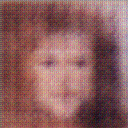
\includegraphics[width=150px]{500_fake_images/samples_5_349.png}%
\caption{A Man With A Beard Wearing A Tie}%
\end{figure}

%
\end{document}